% !TeX spellcheck = sk_SK-Slovak
% !TEX root = szz_mva_main.tex
%%%======= Balicky ======%%
%\documentclass[12pt,a4paper]{sablonaMVA}
%\usepackage{graphicx}
%\usepackage{multirow}
%\usepackage{multicol}
%\usepackage{array}
%\usepackage{lipsum}
%\usepackage{blindtext}
%\usepackage{nicematrix}
%\usepackage{wrapfig}
%\usepackage{caption}
%\usepackage{subcaption}
%\usepackage{amsmath}
%\usepackage{float}
%\usepackage{amssymb}
%\usepackage{hyperref}
%\usepackage{siunitx}
%\usepackage{relsize}
%\sisetup{detect-all}
%\usepackage[english,slovak]{babel}  \usepackage[T1]{fontenc}
%\usepackage{booktabs}
%\usepackage{makecell}
%\usepackage{numerica}
%\usepackage[normalem]{ulem}
%\usepackage{tikz}
%\usepackage{etoolbox}
%\usepackage{enumitem}
%\preto\tabular{\shorthandoff{-}}
%
%%====== Vyplňte údaje ======
%%\documentclass[a4paper,12pt]{article}
%%\usepackage[a4paper,margin=2cm]{geometry}
%\usepackage[most]{tcolorbox}
%\usepackage{xcolor}
%\usepackage{ragged2e}
%
%\newcommand{\uloosdot}[1]{%
%	\tikz[baseline=(todotted.base)]{
%		\node[inner sep=1pt,outer sep=0pt] (todotted) {#1};
%		\draw[loosely dotted] (todotted.south west) -- (todotted.south east);
%	}%
%}%
%
%\begin{document}
% ===================== HLAVIČKA DOKUMENTU =====================
% Definícia farieb podľa predlohy
%\definecolor{nadpisblue}{RGB}{18,32,115}
%\definecolor{boxgray}{RGB}{230,230,230}
%\definecolor{boxborder}{RGB}{90,110,180}

% Pravý horný roh
%\begin{flushright}
%	\small
%	\textbf{BPC-MVT, Mikrovlnná technika}\\
%	Vypracované otázky k SZZ od družiny vajčakov  
%\end{flushright}
%\justifying
%%\vspace*{-10mm}
% ===============================================================
%\section{\normalsize OTÁZKY}
%	\begin{itemize}
%		\item[1.] Základní typy mikrovlnných integrovaných obvodů (hybridní, monolitické MIO, MIO se soustředěnými parametry). Vlnovod integrovaný do substrátu, jeho provedení a základní vlastnosti.
%		Všechny potřebné údaje jsou uvedeny v příloze Důležité údaje a čísla.   
%		%\vspace*{-1.5mm}
%		\item[2.] Rezonátory (rezonátory z úseků vedení, dutinové rezonátory, planární a dielektrické rezonátory). Zásady buzení vlnovodů a dutinových rezonátorů sondou, proudovou smyčkou a štěrbinou.
%		%\vspace*{-1.5mm} 
%		\item[3.] Výkonové děliče, směrové vazební členy a jejich základní technické parametry.
%	\end{itemize}ň
\part{BPC-MVT - Mikrovlnná technika}
%\chapter{Okruhy:}

{\huge Otázky:}

\begin{enumerate}
	\item \textbf{Základní typy mikrovlnných integrovaných obvodů} (\hyperref[tema:HMIO]{hybridní}, \hyperref[tema:MMIO]{monolitické MIO}, \hyperref[tema:MIO_sus_param]{MIO se soustředěnými parametry}). \hyperref[tema:SIW]{Vlnovod integrovaný do substrátu}, jeho provedení a základní vlastnosti.
	
	\item \textbf{Rezonátory} (\hyperref[rez:usek_vedeni]{rezonátory z úseků vedení}, \hyperref[rez:dutinove_rez]{dutinové rezonátory}, \hyperref[rez:planar_rezon]{planární} a \hyperref[rez:dielec_rezon]{dielektrické rezonátory}). Zásady \hyperref[budenie:vlnovod:dutin]{buzení vlnovodů a dutinových rezonátorů} sondou, proudovou smyčkou a štěrbinou.
	
	\item \hyperref[delice]{\textbf{Výkonové děliče}}, \hyperref[odbnocnice]{směrové vazební členy} a jejich \hyperref[odbnocnice_param]{základní technické parametry}.
\end{enumerate}

\newpage

% 	\section{\normalsize \begin{itemize}\item[1.] Základní typy mikrovlnných integrovaných obvodů (\hyperref[tema:HMIO]{hybridní} , \hyperref[tema:MMIO]{monolitické MIO}, \hyperref[tema:MIO_sus_param]{MIO se soustředěnými parametry}). \hyperref[tema:SIW]{Vlnovod integrovaný do substrátu}, jeho provedení a základní vlastnosti. \end{itemize}}
\section{1. okruh}
%\raggedright
	\section{Mikrovlnný integrovaný obvod (MIO):} \label{tema:MIO}
	%\vspace*{2mm}
	\begin{itemize}[label=--]
	%\vspace*{-4mm}
	\item typ integrovaného obvodu pracujúceho v pásme mikrovlnných frekvencií, tvorený prevážne planárnymi štruktúrami
	%\vspace*{-2.5mm}
	\item obvody väčšinou zlučujú činnosti viacero dielčích obvodov (mixéry, zosilnenie, spínanie...) spojených vo vnútri MIO bez prístupu užívateľa
	\end{itemize}
	\bigskip

\begin{tabular}{p{8cm} p{8cm}}
	
	\textbf{Výhody MIO:} & \textbf{Nevýhody MIO:} \\

	\begin{minipage}[t]{8cm}
		%\vspace*{-2mm}
		\begin{itemize}[label=$\oplus$]
			\item planárne usporiadanie obvodov
			%\vspace*{-3.5mm}
			\item malé rozmery a hmotnosť
			%\vspace*{-3.5mm}
			\item nízka spotreba surovín (kovov, polovodičov..)
			%\vspace*{-3.5mm}
%			\item menšia pracnosť, vyššia reprodukovateľnosť výroby, sériovosť, nižšie
%			výrobné náklady
%			%\vspace*{-4mm}
			\item vyššia spoľahlivosť a stabilnosť parametrov obvodu
			%\vspace*{-3.5mm}
			\item väčšia širokopásmovosť obvodov
%			%\vspace*{-4mm}
%			\item kompatibilnosť montáže s polovodičovými prvkami
		\end{itemize}
	\end{minipage}
	&
	\begin{minipage}[t]{8cm}
		%\vspace*{-2mm}
		\begin{itemize}[label=$\ominus$]
			\item väčší merný útlm, nižší činiteľ jakosti obvodov
			%\vspace*{-3.5mm}
			\item menšia elektrická pevnosť, nižší prenášaný výkon
			%\vspace*{-3.5mm}
%			\item horší odvod tepla, problematická integrácia výkonových prvkov
%			%\vspace*{-4mm}
%			\item obtiažnejší návrh obvodov CAD
%			%\vspace*{-4mm}
			\item náročná a precízna technológia
			%\vspace*{-3.5mm}
			\item nemožnosť dodatočných úprav a opravy
%			%\vspace*{-4mm}
%			\item obmedzenie miniaturizáciou a integráciou obvodov
		\end{itemize}
	\end{minipage}
	%\vspace*{5mm}
\end{tabular}

\begin{figure}[H]
	\makebox[\textwidth]{%
		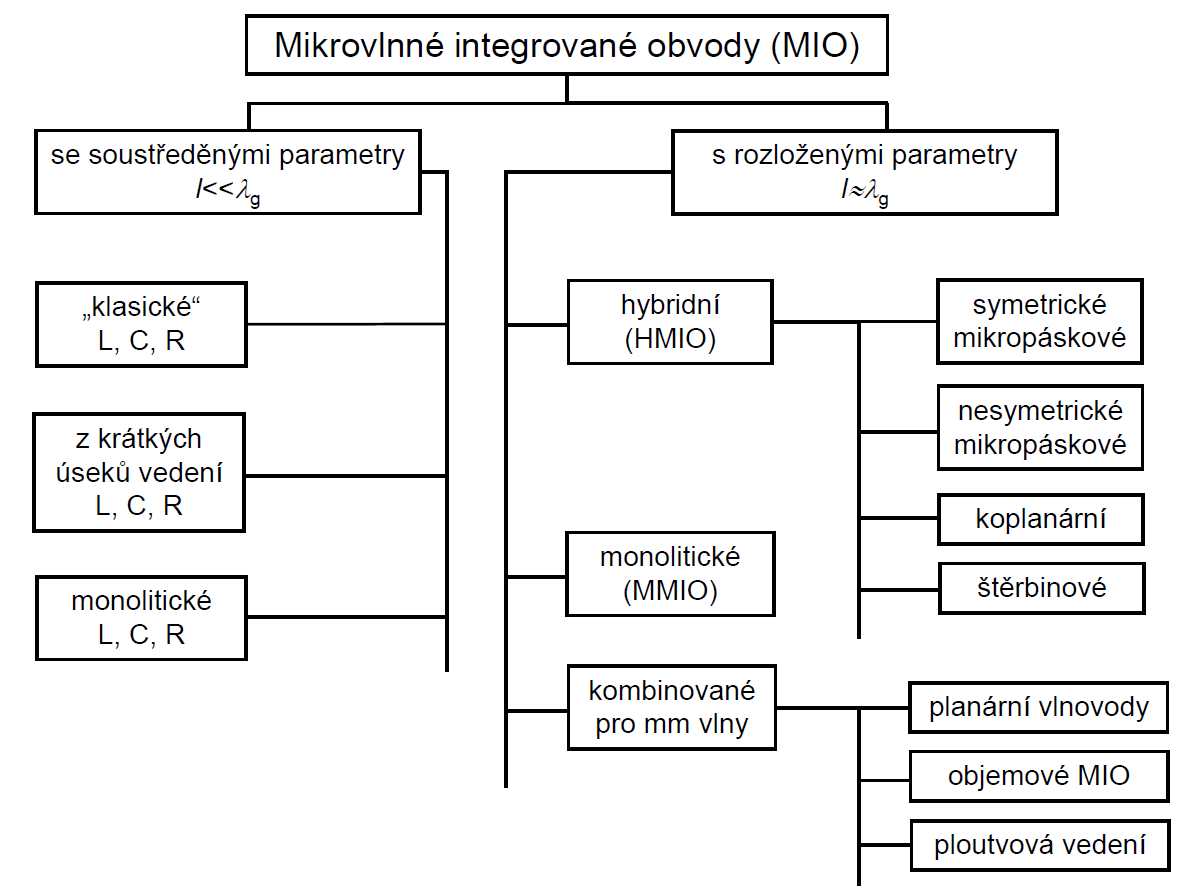
\includegraphics[scale=0.3]{Obrazky/MVT/rozdelenie_mio.png}}
	\caption{Rozdelenie mikrovlnných integrovaných obvodov}
\end{figure}

\section{Hybridné mikrovlnné integrované obvody (HMIO):} \label{tema:HMIO}
%\vspace*{2mm}
\begin{itemize}[label=--]
	%\vspace*{-4mm}
	\item pasívne obvody sa vytvárajú nanesením vodivých páskov na substrát vo tvare vytváraného obvodu (vodivého motívu)
	%\vspace*{-2.5mm}
	\item súčiastky sa do obvodu vkladajú ako diskrétne prvky (pájením alebo ultrazvukovým zváraním)
	%\vspace*{-2.5mm}
	\item umožňujú vzájomne nezávislú optimalizáciu použitých aktívnych súčiastok a pasívnych obvodov
	%\vspace*{-2.5mm}
	\item predstavujú najrozšírenejšiu a bežne využívanú formu mikrovlnnej integrácie
\end{itemize}

\newpage
Základné rozdelenie pasívnych hybridných mikrovlnných integrovaných štruktúr (HMIO štruktúry): 

\begin{figure}[H]
	
	\centering
	\begin{minipage}{0.45\textwidth}
		\centering
		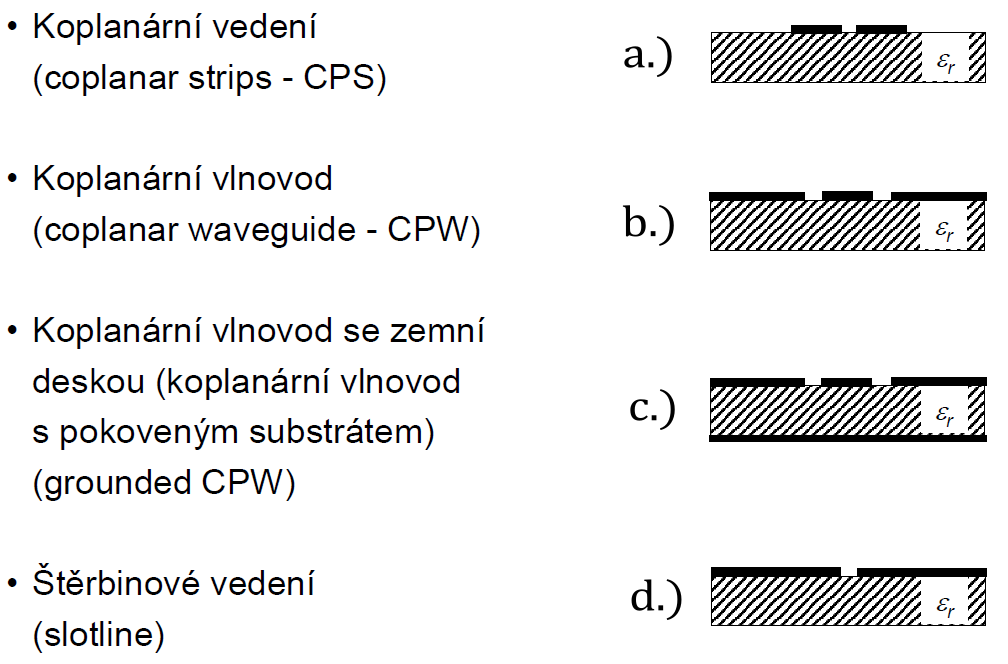
\includegraphics[scale=0.315]{Obrazky/MVT/HMIO_struktury2.png}
	\end{minipage}
	\hspace{12.5mm}
	\begin{minipage}{0.45\textwidth}
		%\vspace{-23.5mm}
		\centering
		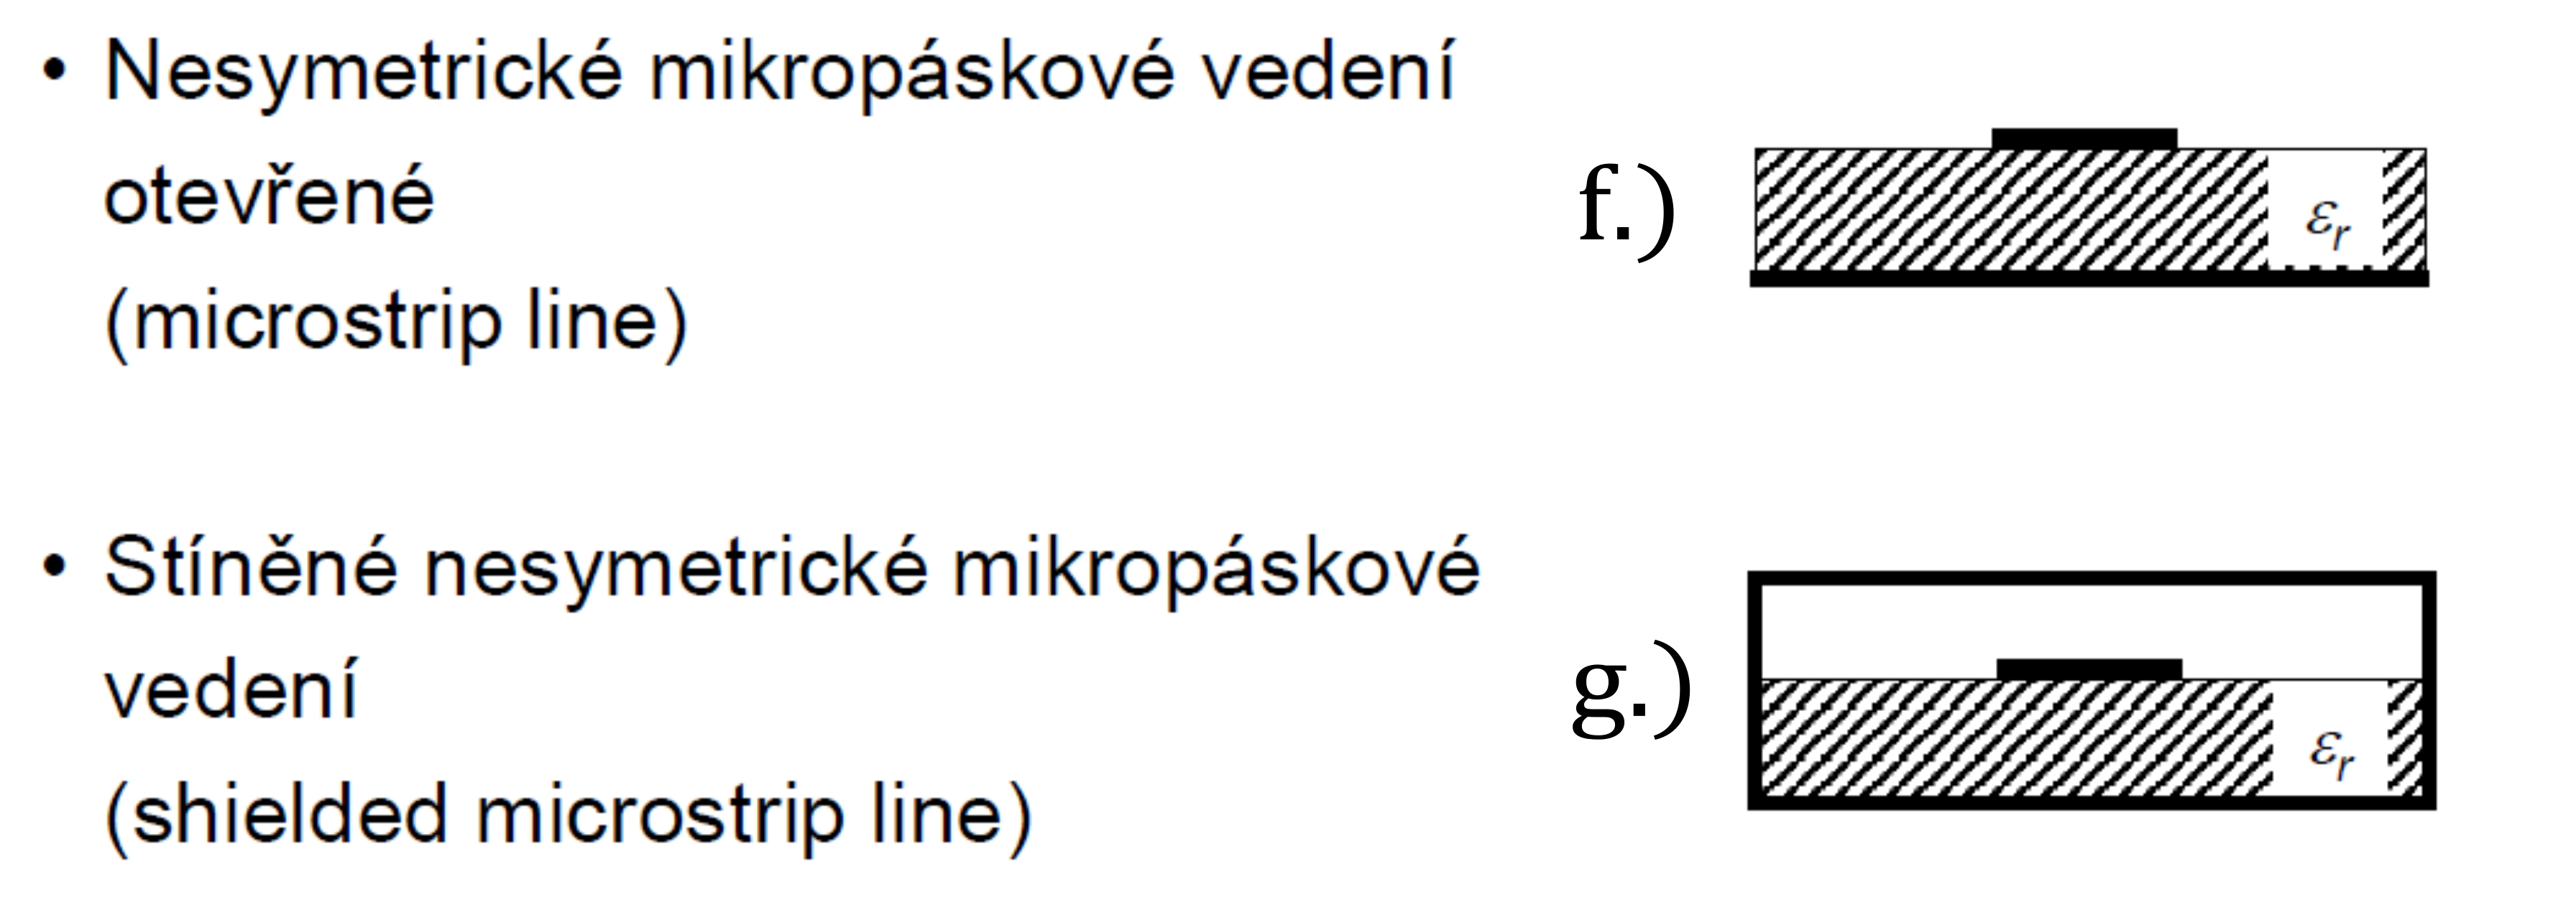
\includegraphics[scale=0.315]{Obrazky/MVT/HMIO_struktury1_b.png}
	\end{minipage}
	%\vspace{2mm}
	\begin{minipage}{0.45\textwidth}
		%\vspace{0mm}
		\hspace{-4cm}
		\centering
		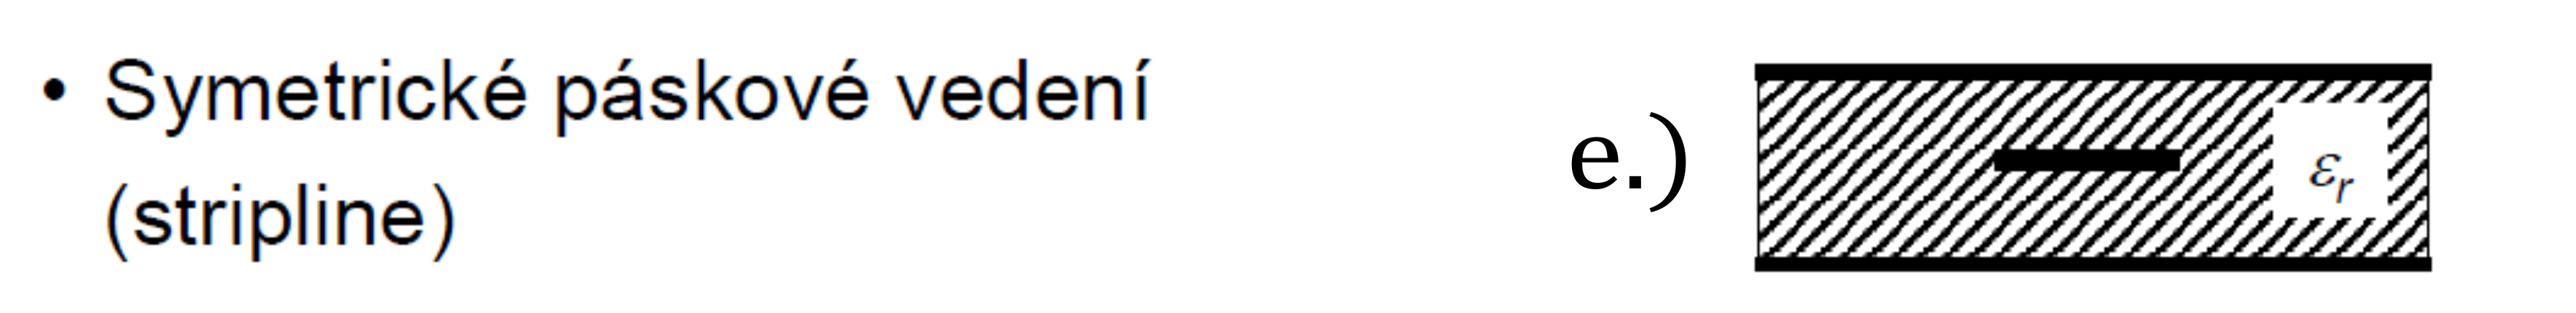
\includegraphics[scale=0.315]{Obrazky/MVT/HMIO_struktury1_a.png}
	\end{minipage}
	\hspace{-10mm}
	\begin{minipage}{0.30\textwidth}
		%\vspace{-25mm}
		\hspace{-15mm}
		\centering
		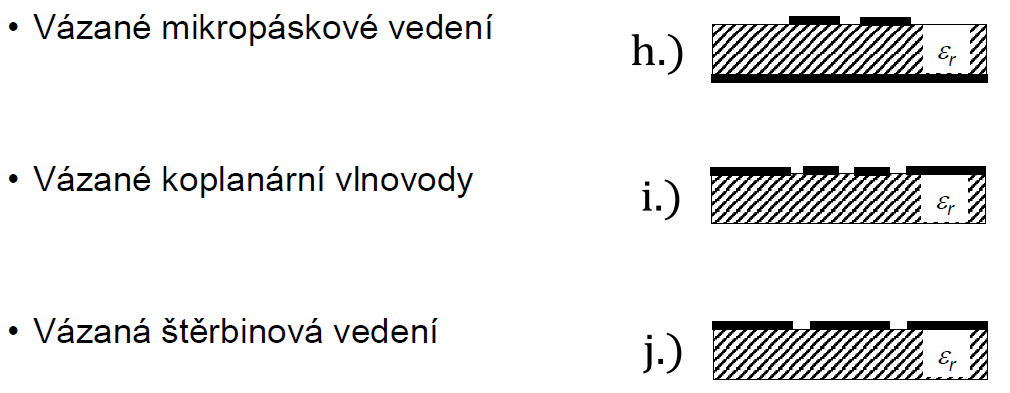
\includegraphics[scale=0.315]{Obrazky/MVT/HMIO_struktury3.png}
	\end{minipage}
	%\vspace{2mm}
	\caption{Základné typy HMIO štruktúr}
	\label{fig:hmio_struktury}
\end{figure}

	\bigskip
	\textbf{Popis symetrického páskového vedenia (stripline) \ref{fig:hmio_struktury}.e.)}
	\begin{itemize}[label=$\rightarrow$]
		%\vspace*{-4mm}
		\item signálový pások je ``utopený'' uprostred dielektrika a z oboch vonkajších strán je zemná plocha
		%\vspace*{-2.5mm}
		\item je schopný prenášať vid TEM
		%\vspace*{-2.5mm}
		\item vďaka tejto konštrukcii sa z neho nemôže šíriť elektromagnetické pole do okolia (nízke vyžarovanie) a nedostáva sa do neho rušenie z vonku
	\end{itemize}
	
	\textbf{Popis neysmetrického mikropáskového vedenia otvoreného (microstrip line) \ref{fig:hmio_struktury}.f.)}
	\begin{itemize}[label=$\rightarrow$]
	%\vspace*{-4mm}
	\item najrozšírenejší typ rovinného prenosového vedenia
	%\vspace*{-2.5mm}
	\item z hornej strany nie je zemná plocha
	%\vspace*{-2.5mm}
	\item elektromagnetická vlna zasahuje z časti do dielektika a z časti do vzduchu (2 rôzne prostredia s  rôznou rýchlosťou šírenia), mikropáskom sa šíri vid kvazi-TEM
	\end{itemize}
	
	\textbf{Popis koplanárneho vedenia (\ref{fig:hmio_struktury}.a.) a koplanárneho vlnovodu (\ref{fig:hmio_struktury}.b.)}
	\begin{itemize}[label=$\rightarrow$]
		%\vspace*{-4mm}
		\item všetky vodivé cesty (signál aj zem) ležia (koplanárne) v jednej rovine na hornej strane dielektrického substrátu
		%\vspace*{-2.5mm}
		\item výhoda je, že všetky diskrétne súčiastky je možné mať v jednej rovine na hornej strane substrátu
		%\vspace*{-2.5mm}
		\item \textbf{vedenie}: elektromagnetické pole je iba medzi 2 páskami (väčšie vyžarovanie do okolia $\rightarrow$ väčšie straty)
		%\vspace*{-2.5mm}
		\item \textbf{vlnovod}: signálový pások je medzi 2 zemnými plochami (elektrické pol je držané vo vnútri medzier $\rightarrow$ zníženie strát do okolia $\rightarrow$ vhodné pre vysoké frekvencie)
	\end{itemize}

	Výber substrátu je ovplyvnený: kmitočtovým pásmom, použitými konektormi, rozmermi komponentov, cenou, relatívnou permitivitou $\varepsilon_r$ a stratovým činiteľom tg $\delta$, teplotnou vodivosťou...\par 
	
	\textbf{Technológia výroby:}
	%\vspace*{2mm} 
	\begin{itemize}[label=--]
		%\vspace*{-4mm}
		\item \textbf{Tenkovrstvá technologia} --  vysoká presnosť výroby ($\pm$5 $\mu$m), nízky útlm
		%\vspace*{-2.5mm}
		\item \textbf{Tlustovrstvá technologia} -- jednoduchá výroba, väčší útlm na vyšších $f$
		%\vspace*{-2.5mm}
		\item \textbf{Leptacia technologia} -- lacná technologická výroba
	\end{itemize}
	
	\textbf{Základné problémy riešenia planárných štruktúr:}
	 %\vspace*{2mm} 
	 \begin{itemize}[label=--]
	 	%\vspace*{-4mm}
	 	\item \textbf{1.} Veľké rozptylové elektromagnetické pole okolo páskových vodičoch (\textbf{nie je možné zanedbať})
	 	%\vspace*{-2.5mm}
	 	\item \textbf{2.} Nehomogenita prostredia (štruktúry sú z časti na vzduchu z časti v substráte)
	 	\begin{itemize}[label=$\rightarrow$]
 			%\vspace*{-2.5mm}
	 		\item  šírenie hybridnej elektromagnetickej vlny \textbf{HEM} s disperziou - \textbf{nie je možné riešiť analyticky} 
 		\end{itemize}
	 \end{itemize}
	\textbf{Možné postupy riešenia:}
	%\vspace*{2mm} 
	\begin{itemize}[label=--]
		%\vspace*{-4mm}
		\item \textbf{Presné riešenie} $\rightarrow$ vlnové rovnice pre vlnu HEM numericky (integrálne rovnice, Galerkinova metóda...)
		%\vspace*{-2.5mm}
		\item \textbf{Aproximácie} $\rightarrow$ aproximácia presných výsledkov jednoduchými matematickými funkciami
		%\vspace*{-2.5mm}
		\item \textbf{Približne riešenie} $\rightarrow$ namiesto vlny HEM sa počíta s kvazi-TEM vlnou, riešenie: pomocou metódy konformného zobrazenia (častá v praxi) 
	\end{itemize}

	\textbf{Popis riešenia 1. problému nesymetrického mikropáskového vedenia metódou konformného zobrazenia:}
	%\vspace{1mm}
	\begin{itemize}[label=$\rightarrow$]
		%\vspace*{-4mm}
		\item predpokladá sa, že celý priestor okolo vodivého pásu je vyplnený rovnakým prostredím (typicky vzduch $\varepsilon_r$ = 1)
		%\vspace*{-2.5mm}
		\item prostredie je tak homogénne (rovnaké) -- šírenie vlny TEM, metódou konformného zobrazenia sa vyrieši Laplaceova rovnica (a spočíta sa základná kapacita vzduchového vedenia)
	\end{itemize}

	
	\begin{figure}[H]
		\makebox[\textwidth]{%
			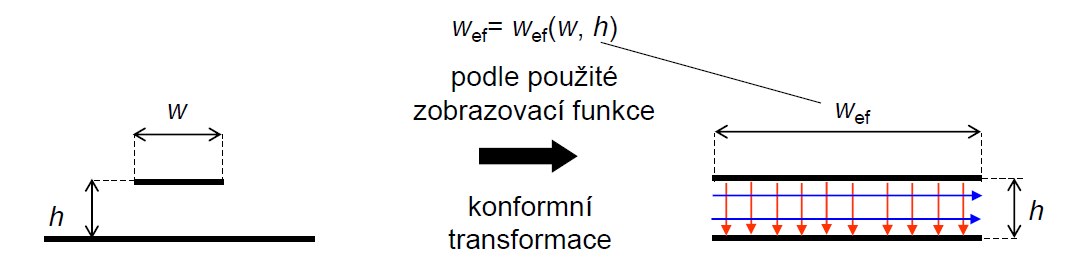
\includegraphics[scale=0.375]{Obrazky/MVT/HMIO_riesenie1_problem.png}}
		\caption{Konformná transformácia 1. problému}
	\end{figure}
	
	Všetky parametre nesymetrického páskového vedenia sa určujú ako
	parametre jeho konformne združeného obrazu bez rozptylového poľa
	a prepočítajú sa späť do pôvodnej štruktúry\par
	\bigskip
	
	\textbf{Popis riešenia 2. problému nesymetrického mikropáskového vedenia metódou konformného zobrazenia:}
	%\vspace{1mm}
	\begin{itemize}[label=$\rightarrow$]
		%\vspace*{-4mm}
		\item Hybridnú elektromagnetickú vlnu HEM je možné na nízkych mikrovlnných kmitočtoch aproximovať vlnou kvazi-TEM (prostredie je nehomogénne)
		%\vspace*{-2.5mm}
		\item priečna nehomogennosť mikropáskového vedenia na dielektrickej podložke sa rešpektuje zavedením pojmu \textbf{efektívna permitivita }
		%\vspace*{-2.5mm}
		\item rozdelenie štruktúry na 2 polovice (vzduch + dielektrikum) 
	\end{itemize}
	
	\begin{figure}[H]
	\makebox[\textwidth]{%
		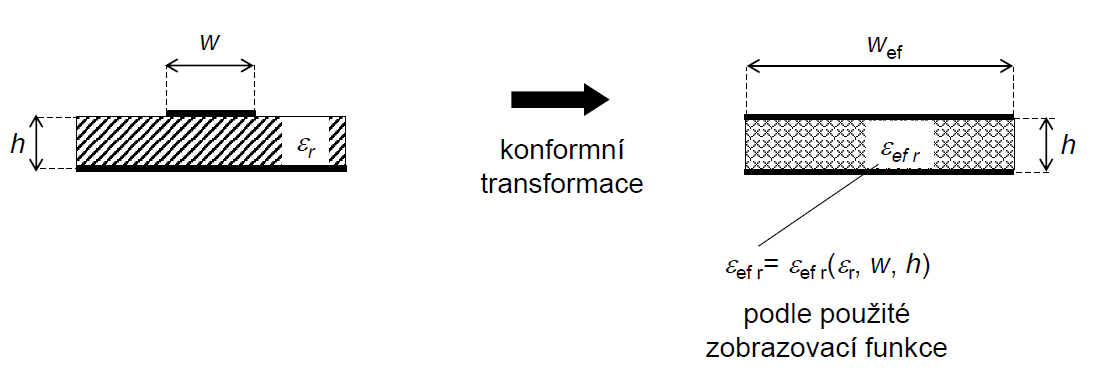
\includegraphics[scale=0.375]{Obrazky/MVT/HMIO_riesenie2_problem.png}}
	\caption{Konformná transformácia 2. problému}
	\end{figure}
	
	\section{MIO so sústredenými parametrami:} \label{tema:MIO_sus_param}
	%\vspace*{2mm}
	\begin{itemize}[label=--]
		%\vspace*{-4mm}
		\item typ obvodu, ktorého fyzické rozmery všetkách súčiastok v obvode sú mnohonásobne (aspoň o rad) menšie než vlnová dĺžka signálu $\lambda_g$ (l $\ll$ $\lambda_g$)
		%\vspace*{-2.5mm}
		\item hovorím o obvode so sústredenými parametrami, ak jeho rozmery nepresiahnu hodnotu~$\lambda$/10
		%\vspace*{-8mm}
		\item súčiastky sú tvorené pomocou planárnych metód (napr. vyleptávaním)
	\end{itemize}
	
	\begin{tabular}{p{8cm} p{8cm}}
		
		\textbf{Výhody:} & \textbf{Nevýhody:} \\
		
		\begin{minipage}[t]{8cm}
			%\vspace*{-2mm}
			\begin{itemize}[label=$\oplus$]
				\item vysoký stupeň integrácie a miniaturizácie 
				%\vspace*{-3.5mm}
				\item malá váha a nízka spotreba materiálov
				%\vspace*{-8.5mm}
				\item dobrá reprodukovateľnosť, vysoká sériovosť výroby $\rightarrow$ nízka cena
				%\vspace*{-3.5mm}
				\item jednoduchosť konštrukcie $\rightarrow$ vysoká spoľahlivosť
				%\vspace*{-3.5mm}
				\item veľká širokopásmovosť (el. vlastnosti sa neopakujú s kmitočtom)
			\end{itemize}
		\end{minipage}
		&
		\begin{minipage}[t]{8cm}
			%\vspace*{-2mm}
			\begin{itemize}[label=$\ominus$]
				\item náročná (miniatúrna) technológia
				%\vspace*{-3.5mm}
				\item značné straty v obvode vplyvom parazitných vlastností, nízke Q
				%\vspace*{-3.5mm}
				\item obmedzenie pracovného pásma kmitočtu zhora (dosažiteľnosť malých rozmerov, klesajúcej hodnoty Q, zmeny charakteru prvku)
			\end{itemize}
		\end{minipage}
		%\vspace*{5mm}
	\end{tabular}
	
	\section{Induktory:}
	\textbf{V klasickej podobe}
	%\vspace*{-2.5mm}
	\begin{itemize}[label=$\rightarrow$]
		\item planárne špirály, meandre tvorené tenkým (vodivým) pásikom na substráte ($L$ jednotky a stovky nH, $Q$ $\approx$ 100)
		%\vspace*{-3.5mm}
		\item indukcia vzniká predĺženým prúdovej dráhy a magnetickým poľom $H$ v okolí vodiča.
	\end{itemize}
	
	\begin{figure}[H]
		\makebox[\textwidth]{%
			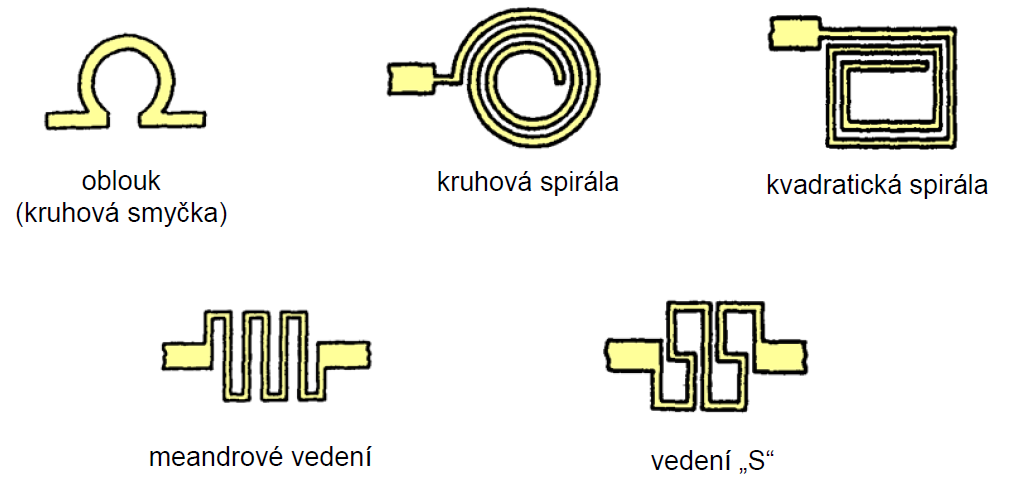
\includegraphics[scale=0.375]{Obrazky/MVT/induktory_klasicke.png}}
		\caption{Prevedenia induktorov v klasickej podobe}
	\end{figure}
	{\raggedright \textbf{Z veľmi krátkych úsekov vedení}}\\
	%\vspace*{-2.5mm}
	$\rightarrow$ zúžením planárneho vodiča (nespráva sa ako normálne vedenie, ale ako sériová indukčnosť)
	\begin{figure}[H]
		\makebox[\textwidth]{%
			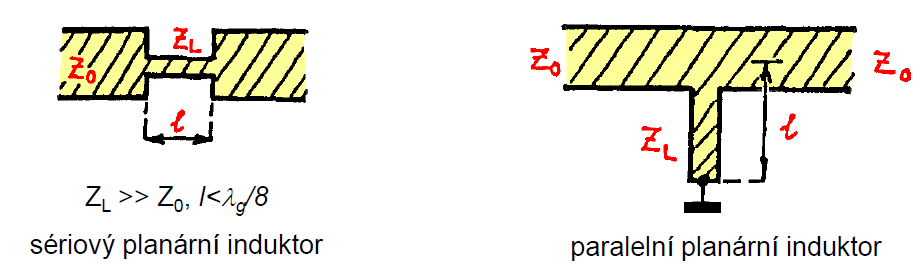
\includegraphics[scale=0.375]{Obrazky/MVT/induktory_useky_vedenia.png}}
		\caption{Prevedenia induktorov z krátkych úsekov vedenia}
	\end{figure}
	
	\section{Kapacitory:}
	\textbf{V klasickej podobe} \\
	%\vspace*{-2.5mm}
	$\rightarrow$ realizácia medzerou v mikropásku ($C$ stotiny až stovky pF, $Q$ niekoľko stoviek)
	\begin{figure}[H]
		\makebox[\textwidth]{%
			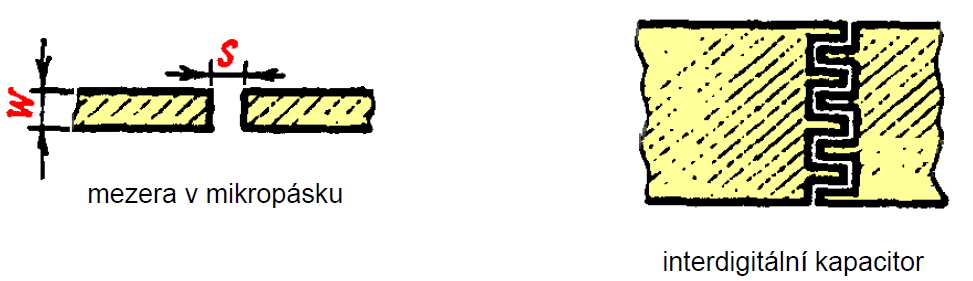
\includegraphics[scale=0.375]{Obrazky/MVT/kapacitory_klasicke.png}}
		\caption{Prevedenia kondenzátorov v klasickej podobe}
	\end{figure}
	{\raggedright \textbf{Z veľmi krátkych úsekov vedení}}\\
	%\vspace*{-2.5mm}
	$\rightarrow$ zväčšením šírky pásku (opačne ako u induktora)
	\begin{figure}[H]
		\makebox[\textwidth]{%
			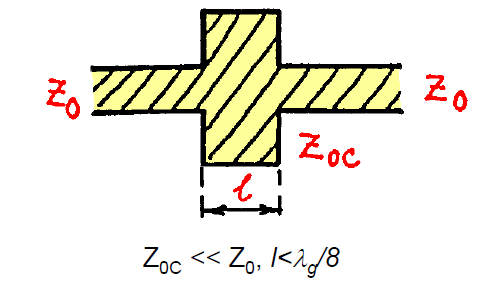
\includegraphics[scale=0.375]{Obrazky/MVT/kapacitory_useky_vedenia.png}}
		\caption{Prevedenia kondenzátorov z krátkych úsekov vedenia}
	\end{figure}
	
	\section{Rezistory:}
	%\vspace*{-2mm}
	\begin{itemize}[label=$\rightarrow$]
		\item pomocou planárnych tenkých odporových vrstiev (nanesením tenkého filmu (NiCr, Ta2N) z odporového materiálu na substrát)
		%\vspace*{-3.5mm}
		\item pre menšie a stredné odpory (9,5 až 135 $\Omega$)
	\end{itemize}
	
	\begin{figure}[H]
		\makebox[\textwidth]{%
			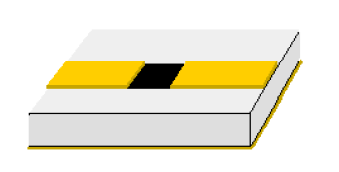
\includegraphics[scale=0.4]{Obrazky/MVT/rezistory.png}}
		\caption{Prevedenie rezistora so sústredeným odporom}
	\end{figure}
	
	\section{Monolitické mikrovlnné integrované obvody (MMIO):} \label{tema:MMIO}
	%\vspace*{2mm}
	\begin{itemize}[label=--]
		%\vspace*{-4mm}
		\item pasívne a aktívne obvodové prvky, ktorých spojenia a mikropáskové vedenia sú vytvorené \textbf{na povrchu} alebo \textbf{v objemu} polovodičového substrátu, ktorý plní funkcie
			\begin{itemize}[label=$\rightarrow$]
				%\vspace{-2.5mm}
				\item \textbf{nosná (dielektrická) podložka} pre prenosové vedenia, obvodové elementy s rozloženými parametrami a hybridnými prvkami so sústredenými 
				%\vspace{-2mm}
				\item \textbf{blok polovodiča pre vytváranie} a monolitickú integráciu aktívnych a pasívnych polovodičových súčiastok
			\end{itemize} 
		%\vspace*{-3.5mm}
		\item predstavujú najvyšší stupeň mikrovlnnej integrácie a sú bežne využívane, stále prebieha vývoj
	\end{itemize}
	
	
	\begin{tabular}{p{8cm} p{8cm}}
	\textbf{Výhody MIO:} & \textbf{Nevýhody:} \\
	
	\begin{minipage}[t]{8cm}
		%\vspace*{-2mm}
		\begin{itemize}[label=$\oplus$]
			\item malá hmotnosť a rozmery
			%\vspace*{-3.5mm}
			\item jednoduchá výroba ďalších FETov v MMIO
			%\vspace*{-3.5mm}
			\item podstatne menšie parazitné reaktancie v porovnaní s diskrétnymi súčiastkami
			%\vspace*{-7.5mm}
			\item veľká reprodukovateľnosť výroby
		\end{itemize}
	\end{minipage}
	&
	\begin{minipage}[t]{8cm}
		%\vspace*{-2mm}
		\begin{itemize}[label=$\ominus$]
			\item veľká spotreba drahého polovodiča pre prenosové vedenie
			%\vspace*{-3.5mm}
			\item náročná a drahá výroba (hlavne pre malé  série)
			%\vspace*{-3.5mm}
			\item náročný návrh MMIO kvôli toleranciám výrobnej 
			%\vspace*{-3.5mm}
			\item nemôžu byť použité pre veľké výkony
			%\vspace*{-3.5mm}
			\item veľmi ťažká implementácia obvodov s vysokým činiteľom
		\end{itemize}
	\end{minipage}
	%\vspace*{5mm}
	\end{tabular}
	
	%\vspace{-5mm}
	\subsubsection{Materály pre MMIO}
	Ako materiály sa používajú kremík \textbf{Si} (pre nižšie $f$ a výkonové aplikácie), arzenid gália \textbf{GaAs} (najpoužívanejší), fosfid india \textbf{InP} (pre pásma mm vĺn)...
	
	\subsubsection{Výhody GaAs}
		%\vspace*{-2mm}
	\begin{itemize}[label=$\oplus$]
		\item 6$\times$ väčšia pohyblivosť elektrónov než \textbf{Si} a 2x vyššia maximálna driftová rýchlosť (preletová doba elektrónov je kratšia $\rightarrow$ možnosť práce na vyšších $f$)
		%\vspace*{-3.5mm}
		\item 6$\times$ -- 4$\times$ väčší merný odpor než izolačný \textbf{SISi}
		%\vspace*{-3.5mm}
		\item stabilnosť parametrov v procesu technologického spracovania6x -- 4x väčší merný odpor než izolačný \textbf{SISi}
		%\vspace*{-3.5mm}
		\item väčšia šírka zakázaného pásma (vysoká tepelná odolnosť, možnosť práce s vysokými výkonmi)
	\end{itemize}
	
	\subsubsection{Nevýhody GaAs}
	%\vspace*{-2mm}
	\begin{itemize}[label=$\ominus$]
		\item Drahý východzí materiál (gálium)
		%\vspace*{-3.5mm}
		\item Veľmi drahá a zložitá technológia
		%\vspace*{-3.5mm}
		\item Asi 3$\times$ menšia tepelná vodivosť \textbf{GaAs} než u \textbf{Si}
			\begin{itemize}[label=$\rightarrow$]
			%\vspace{-2.5mm}
			\item zlý odvod tepla 
			%\vspace{-2mm}
			\item problémy s integráciou výkonových prvkov
		\end{itemize} 
	\end{itemize}

	\subsubsection{Návrh a výroba MMIO}
%\vspace*{-2mm}
\begin{itemize}[label=--]
	\item Návrh MMIO vyžaduje použitie CAD programov, postup výroby:
	\begin{itemize}[label=$\downarrow$]
	%\vspace*{-3mm}
	\item vytvorenie aktívnej vrstvy pol. substrátu pre aktívne prvky
	%\vspace*{-1.5mm}
	\item  izolácia aktívnych prvkov (+ ponechanie dostatočnej maksy pre aktívne prvky)
	%\vspace*{-1.5mm}
	\item vytvorenie ohmických kontaktov, dokončenie a testovanie aktívnych prvkov
	%\vspace*{-1.5mm}
	\item vytvorenie metalických vrstiev pre kontakty, prenosové vedenia, induktory...
	%\vspace*{-1.5mm}
	\item úprava zadnej strany substrátu a vytvorenie prechodov spojujúce prvky so zemnou vrstvou
	\end{itemize}
\end{itemize}

\section{Vlnovod integrovaný do substrátu SIW} \label{tema:SIW}
	%\vspace*{2mm}
\begin{itemize}[label=--]
	%\vspace*{-4mm}
	\item dielektrický substrát je z oboch strán pokovený (horná a dolná stena vlnovodu), bočné steny sú tvorené rovnobežnými radami prekovov, spájajúce hornú a dolnú stenu 
	%\vspace*{-2.5mm}
	\item vlastnosti podobné obdĺžnikovému vlnovodu 
	%\vspace*{-2.5mm}
	\item šíri sa v nej len vidy TE$_{m0}$ (TM vidy neexistujú)
\end{itemize}
\bigskip
\begin{figure}[H]
	\makebox[\textwidth]{%
		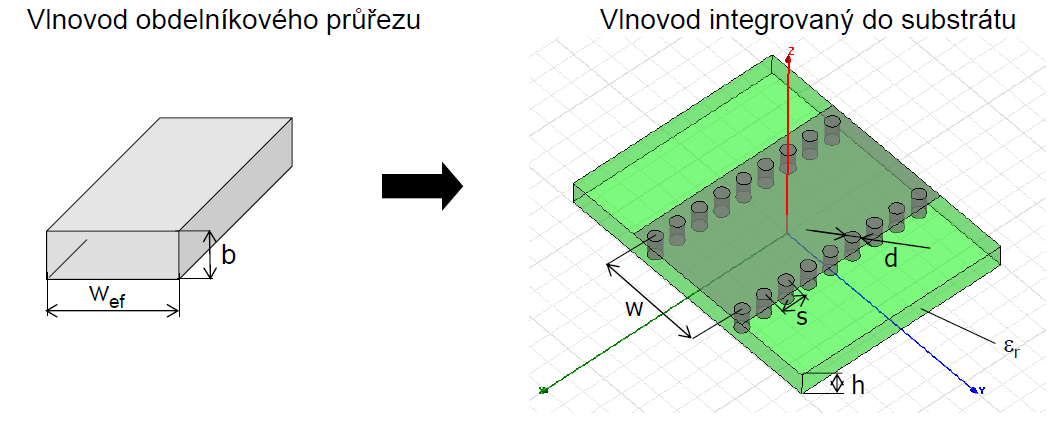
\includegraphics[scale=0.4]{Obrazky/MVT/SIW_prechod.png}}
	\caption{Prechod od vlnovodu obdĺžnikového prierezu do vlnovodu SIW}
\end{figure}

\begin{tabular}{p{8cm} p{8cm}}
	
	\textbf{Výhody:} & \textbf{Nevýhody:} \\
	
	\begin{minipage}[t]{8cm}
		%\vspace*{-2mm}
		\begin{itemize}[label=$\oplus$]
			\item jednoduchá a relatívne lacná výrobná technológia (jak DPS)
			%\vspace*{-3.5mm}
			\item ľahké naviazanie na okolité planárne obvody
			%\vspace*{-3.5mm}
			\item vhodné pre návrh obvodov a antén v pásmu cm a mm vln
		\end{itemize}
	\end{minipage}
	&
	\begin{minipage}[t]{8cm}
		%\vspace*{-2mm}
		\begin{itemize}[label=$\ominus$]
			\item väčší útlm než u vlnovodu obdĺžnikového prierezu (so vzduch. dielektrikom) -- konečná vodivosť stien, straty v dielektriku, malá výška substrátu...
		\end{itemize}
	\end{minipage}
	%\vspace*{5mm}
\end{tabular}

%\section{\normalsize \begin{itemize}\item[2.] Rezonátory (\hyperref[rez:usek_vedeni]{rezonátory z úseků vedení},\hyperref[rez:dutinove_rez]{dutinové rezonátory}, \hyperref[rez:planar_rezon]{planární} a \hyperref[rez:dielec_rezon]{dielektrické rezonátory}). Zásady \hyperref[budenie:vlnovod:dutin]{buzení vlnovodů a dutinových rezonátorů} sondou, proudovou smyčkou a štěrbinou. \end{itemize}}
\section{2. okruh}
	
	Základné typy mikrovlnných rezonátorov:
		%\vspace*{2mm}
	\begin{itemize}[label=--]
		%\vspace*{-4mm}
		\item \textbf{rezonátory z úseku vedení} (mikropáskové, dĺžka $\lambda$/2 alebo $\lambda$/4)
		%\vspace*{-2.5mm}
		\item \textbf{dutinové rezonátory} (kovová dutina, vo vnútri vzniká elektromagnetické pole) 
		%\vspace*{-2.5mm}
		\item \textbf{planárne rezonátory} (priamo na substráte, mikropáskové/šterbinové prevedenie)
		%\vspace*{-2.5mm}	
		\item \textbf{dielektrické rezonátory} (rezonancia vnziká v dielektrickom materiály s vysokým $\varepsilon_r$)
	\end{itemize}
	Parametre rezonátorov sú \textbf{rezonančný kmitočet} a \textbf{činiteľ jakosti}. 
	
	\section{Reznátory s úseku vedení} \label{rez:usek_vedeni}
	%\vspace*{-2mm}
	\section{Vedenie nakrátko}
	%\vspace*{-2mm}
		\begin{itemize}[label=--]
		\item vlna narazí na stenu (skrat) a odrazí sa v protifáze (I = MAX, U = 0)
			\begin{itemize}[label=$\rightarrow$]
			%\vspace*{-3mm}
			\item vedenie nakrátko o dĺžke $\mathbf{\lambda/4}$: správa sa ako \textbf{paralelný} rezonančný obvod (zmena 0 impedancie na konci na $\infty$ impedanciu na začiatku)
			%\vspace*{-1.5mm}
			\item vedenie nakrátko o dĺžke $\mathbf{\lambda/2}$: správa sa ako \textbf{sériový} rezonančný obvod (na vstupe zopakuje skrat z konca)
		\end{itemize}
	\end{itemize}
	
	\section{Vedenie naprázdno} 
	%\vspace*{-2mm}
	\begin{itemize}[label=--]
		\item rezonátor na konci fyzicky rozpojený (I = 0, U = MAX)
		\begin{itemize}[label=$\rightarrow$]
			%\vspace*{-3mm}
			\item vedenie naprázdno o dĺžke $\mathbf{\lambda/4}$: správa sa ako \textbf{sériový} rezonančný obvod (vedenie ma $\infty$ impedanciu)
			%\vspace*{-1.5mm}
			\item vedenie naprázdno o dĺžke $\mathbf{\lambda/2}$: správa sa ako \textbf{paralelný} rezonančný obvod ($\infty$ impedancia na konci $\rightarrow$ 0 impedancia na začiatku)
		\end{itemize}
	\end{itemize}
	
\begin{figure}[H]
	
	\centering
	\begin{subfigure}[t]{0.48\textwidth}
		\centering
		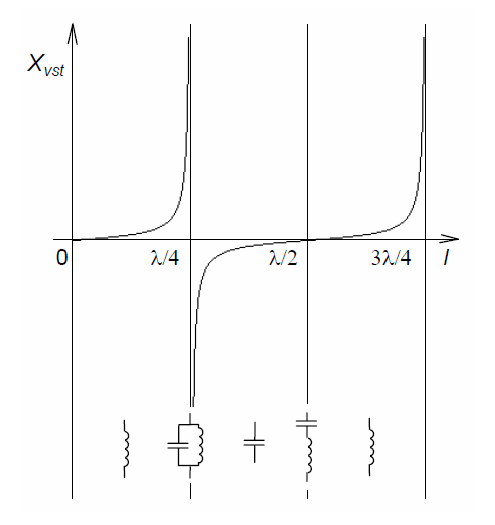
\includegraphics[scale=0.4]{Obrazky/MVT/rezonatory_z_useku_vedeni_nakratko.png}
		\caption{nakrátko}
	\end{subfigure}
	\hspace{2mm}
	\begin{subfigure}[t]{0.48\textwidth}
		\centering
		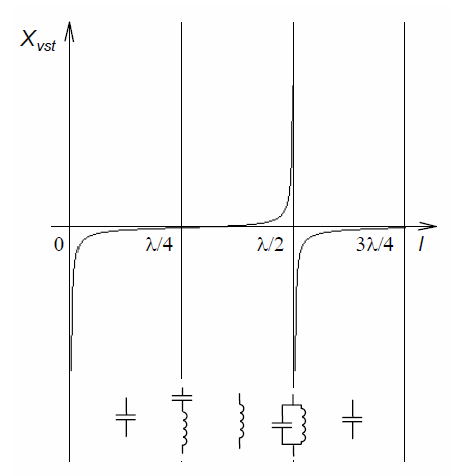
\includegraphics[scale=0.425]{Obrazky/MVT/rezonatory_z_useku_vedeni_naprazdno.png}
		\caption{naprázdno}
	\end{subfigure}
	\caption{Závislosť vstupnej reaktancie úseku vedenia}
	\label{fig:rezonatory}
\end{figure}
	
	\section{Dutinové rezonátory} \label{rez:dutinove_rez}
	%\vspace*{2mm}
	\begin{itemize}[label=--]
		%\vspace*{-4mm}
		\item mikrovlnný rezonančný obvod (uzatvorený vodivý plášť, obsah vyplňuje dielektrikum vzduch/vákuum)
		%\vspace*{-2.5mm}
		\item \textbf{princíp}: odraz elektromagnetickej vlny od stien $\rightarrow$ stojaté vlnenie a silná rezonancia
		%\vspace*{-2.5mm}
		\item majú veľmi vysoký činiteľ jakosti $Q_0$ (radovo $10^3$ až $10^5$) - dôsledkom žiadnych strát vyžarovaním
	\end{itemize}
%	\textbf{Komplexný rezonančný kmitočet} dutinového rezonátoru - (slúži na analýzu strát a rezonancií): 
%	 \begin{equation}
% 	 	\omega = \omega_0 \left(1 - \frac{1}{2Q_0}\right) + j \frac{\omega_0}{2Q_0} = \omega_r + j\frac{\omega_0}{2Q_0}
% 	 \end{equation}
	\textbf{Činiteľ jakosti} nezaťaženého rezonátoru (nepripojeného k vonkajším obvodom - vlastný činiteľ jakosti):
	\begin{equation}
		Q_0 = \frac{\omega_0 W}{P_z}
	\end{equation}
%	 	 $\omega_0$ - uhlový rezonančný kmitočet,\\
%		 $W$ - stredná hodnota celkovej energie elmag. pola v dutine pri rezonancii\\
%		 $P_z$ - stredná hodnota činiteľa výkonu strateného v rezonátore vplyvom strát)\par
%		 \bigskip
	{\raggedright \textbf{Vlastný činiteľ jakosti} vplyvom strát v nedokonalých stenách:}
	\begin{equation}
		Q_0 \approx \frac{2}{\delta}\frac{V}{S_p}
	\end{equation}
%		$V$ - objem dutiny, 
%		$S_p$ - vnútorný povrch plášťa dutiny, 
%		$\delta$ - hĺbka vniku\par
%		\bigskip
%	{\raggedright \textbf{Činiteľ jakosti rezonátora so strátovým dielektrikom} }
%	\begin{equation}
%		 \frac{1}{Q_{0c}} = \frac{1}{Q_0}+tan(\delta)
%	\end{equation}
	\section{Vlnovodové dutinové rezonátory}
		%\vspace{-3mm}
	\begin{itemize}[label=--]
		\item rezonuje na nekonečne mnoho diskrétnych kmitočtoch, pričom každému z nich patrí iné usporiadanie poľa typu \textbf{TM} alebo \textbf{TE} v dutine
		%\vspace{-3.5mm}
		\item vidy \textbf{TM} a \textbf{TE} sú charakterizované tromi vidovými číslami $m$, $n$, $p$
		%\vspace{-3.5mm}
		\item čísla $\mathbf{m}$ a $\mathbf{n}$ určujú typ vidu TM/TE a usporiadanie elektromagnetického poľa
		\begin{itemize}[label=$\rightarrow$]
			%\vspace{-3.5mm}
			\item číslo $\mathbf{m}$ udáva počet polvĺn v smere osy ``x''
			%\vspace{-2.5mm}
			\item číslo $\mathbf{n}$ udáva počet polvĺn v smere osy ``y''
		\end{itemize}
		%\vspace{-5mm}
		\item číslo $\mathbf{p}$ udáva počet polvĺn v smere osy ``z'' (rozloženie poľa v pozdĺžnom smere)
		%\vspace{-3.5mm}
		\item vidy sa označujú ako TE$_{mnp}$ a TM$_{mnp}$
	\end{itemize}
	
	\section{Kvádrové rezonátory}
	\begin{itemize}[label=--]
		%\vspace*{-2.5mm}
		\item sú dutinové rezonátory vytvorené z úseku vlnovodu obdĺžnikového prierezu
		%\vspace*{-3.5mm}
		\item prelaďovanie rezonátora sa robí zmenou jeho dĺžky (jedna čelná strana je realizovaná posuvným skratovacím piestom)
		%\vspace*{-3.5mm}
		\item \textbf{dominantný vid}: TE$_{101}$ (vid ma najnižší rezonančný kmitočet, ktorý nezávisí na výške \textbf{b} kvádrovej dutiny)
		\begin{itemize}[label=$\rightarrow$]
			%\vspace*{-4mm}
			\item $\lambda_{\text{mez}} = 2\cdot a$
		\end{itemize}
	\end{itemize}	
	
	\begin{equation}
		f_0 = \frac{1}{2\pi \sqrt{\varepsilon \mu}} \sqrt{\left(\frac{m\pi}{a}\right)^2+\left(\frac{n\pi}{b}\right)^2+\left(\frac{p\pi}{l}\right)^2}
	\end{equation}
	
	\begin{equation}
		\lambda_0 = \frac{2\pi}{\sqrt{\left(\frac{m\pi}{a}\right)^2+\left(\frac{n\pi}{b}\right)^2+\left(\frac{p\pi}{l}\right)^2}}
	\end{equation}
	
	
	\begin{figure}[H]			
		\centering
		\begin{subfigure}[t]{0.48\textwidth}
			\centering
			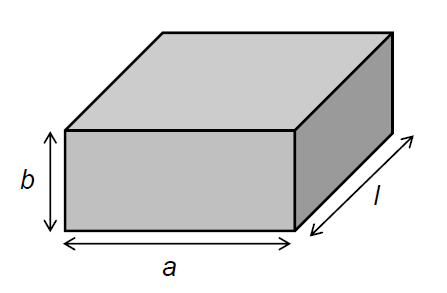
\includegraphics[scale=0.25]{Obrazky/MVT/kvader.png}
			\caption{Kváder}
		\end{subfigure}
			\hspace{-20mm}
		\begin{subfigure}[t]{0.48\textwidth}
			\centering
			\captionsetup{justification=centering}
			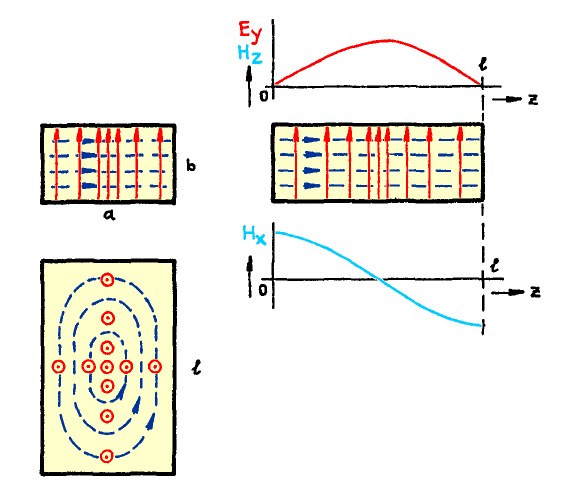
\includegraphics[scale=0.25]{Obrazky/MVT/kvader_elmag.png}
			\caption{Zobrazenie elmag. poľa kvádrového rezonátora}
		\end{subfigure}
			\caption{Kvadrový rezonátor}
			\label{fig:rezonatory_kvader}
	\end{figure}
		
	\section{Válcové rezonátory}
	\begin{itemize}[label=--]
	%\vspace*{-3mm}
	\item najpoužívanejší typ vlnovodu (jednoduchá výroba, výhodné el. a konštrukčné vlastnosti), používa sa aj na presné mikrovlnné vlnomery 
	%\vspace*{-3.5mm}
	\item vysoký vlastný činiteľ jakosti $Q_0$ ($10^3$ až $10^5$)
	%\vspace*{-3.5mm}
	\item môžu vznikať vidy s nulovými číslami typu TM$_{0n0}$
	%\vspace*{-3.5mm}
	\item používajú sa najčastejšie s rotáčne symetrickými vidy (typ: TE$_{0np}$, najčastejšie TE$_{011}$)
	\begin{itemize}[label=$\rightarrow$]
		%\vspace*{-3mm}
		\item kvôli zanedbateľným strátam (siločiary el. poľa tvoria sústredené kružnice a nedotýkajú sa stien, zatiaľ čo prúdy stenami pretekajú)
		%\vspace*{-2mm}
		\item maximálny vlastný činiteľ jakosti Q$_0$ (TE$_{011}$ pri rovnosti $D=2a$)
		%\vspace*{-2mm}
		\item fungujú ako ,,vidový filter'' (zabraňujú vzniku všetkých vidov okrem rotáčne symetrických)
		%\vspace*{-2mm}
		\item s vidom TE$_{011}$ má rezonančná dutina najmenší objem a najväčšiu preladiteľnosť bez degenerácie vidu
		%\vspace*{-2mm}
	\end{itemize}
	\end{itemize}

\begin{figure}[H]			
	\centering
	\begin{subfigure}[t]{0.48\textwidth}
		\centering
		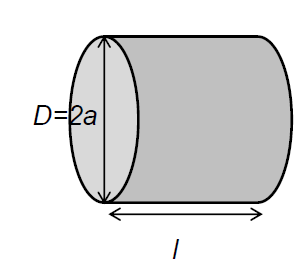
\includegraphics[scale=0.4]{Obrazky/MVT/valec.png}
		\caption{Kváder}
	\end{subfigure}
	\hspace{-20mm}
	\begin{subfigure}[t]{0.48\textwidth}
		\centering
		\captionsetup{justification=centering}
		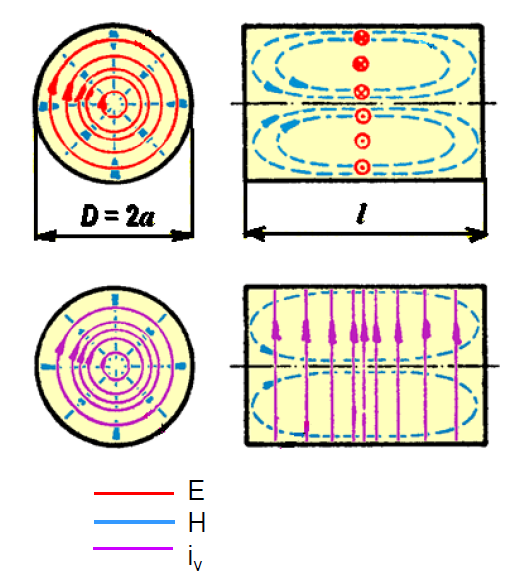
\includegraphics[scale=0.25]{Obrazky/MVT/valec_elmag.png}
		\caption{Zobrazenie elmag. poľa kvádrového rezonátora}
	\end{subfigure}
	\caption{Kvadrový rezonátor}
	\label{fig:rezonatory_valec}
\end{figure}

	\section{Koaxiálne rezonátory}
	\begin{itemize}[label=--]
	%\vspace*{-3mm}
	\item sú tvorené koaxiálnou dutinou, tj. úsekom koaxiálneho vedenia uzavreným na oboch koncoch nakrátko
	%\vspace*{-3.5mm}
	\item fungujú výhradne s vidom \textbf{TEM} (dominantný vid koaxiálneho vedenia)
	%\vspace*{-3.5mm}
	\item väčšinou sa používajú dva druhy koaxiálnych rezonátorov:
	\begin{itemize}[label=$\rightarrow$]
		%\vspace*{-3mm}
		\item \textbf{polvlnné koaxiálne rezonátory}
		%\vspace*{-2mm}
			\item[$\dashrightarrow$] vidové číslo $p$ určuje počet polvĺn elektromagnetického poľa na dĺžke rezonátora
			%\vspace*{-2mm}
			\item[$\dashrightarrow$] základný vid kmitania je pre $p = 1$ 
			%\vspace*{-2mm}
			\item[$\dashrightarrow$] často sa realizuje s mechanickým prelaďovaním pomocou posuvného piesta 
		\item \textbf{štvrťvlnné koaxiálne rezonátory}
			%\vspace*{-2mm}
			\item[$\dashrightarrow$] využíva rezonančných vlastností štvrťvlnného skratovaného vedenia
			%\vspace*{-2mm}
			\item[$\dashrightarrow$] do dutiny se zasúva stredný vodič, na konci stredného vodiča vzniká medzi ním a stenou oproti dutine kapacita $C_0$, ktorá skracuje rezonančnú dĺžku dutiny. 	
	\end{itemize}
	\end{itemize}

	\begin{figure}[H]			
		\centering
		\begin{subfigure}[t]{0.48\textwidth}
			\centering
			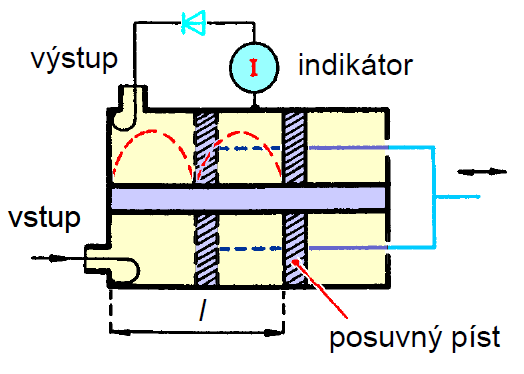
\includegraphics[scale=0.25]{Obrazky/MVT/polvlnny_koax.png}
			\caption{polvlnný}
		\end{subfigure}
		\hspace{-20mm}
		\begin{subfigure}[t]{0.48\textwidth}
			\centering
			\captionsetup{justification=centering}
			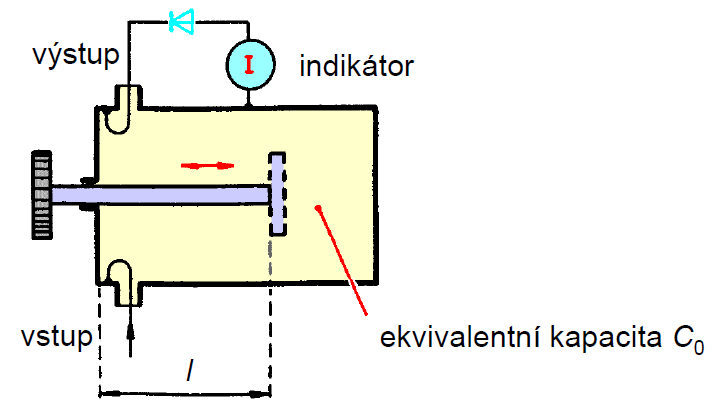
\includegraphics[scale=0.25]{Obrazky/MVT/stvrtvlnny_koax.png}
			\caption{štvrťvlnný}
		\end{subfigure}
		\caption{Koaxiálny rezonátor}
		\label{fig:koaxy}
	\end{figure}
	
	\section{Planárne rezonátory} \label{rez:planar_rezon}
	\begin{itemize}[label=--]
		\item Obdĺžnikový deskový rezonátor
		%\vspace*{-3mm}
		\item Kruhový deskový rezonator
		%\vspace*{-2mm}
		\subitem $\rightarrow$ rezonuje s vidy TE$_{mn0}$ ($m = 0,1,2..., n = 1,2...$) 
		%\vspace*{-2mm}
		\item Prstencový mikropáskový rezonátor a mikropáskový rezonátor z prstencovej vyseče
		%\vspace*{-2mm}
		\subitem $\rightarrow$ rezonuje s vidom kvazi-TEM 
		%\vspace*{-2mm}
		\item Rezonátory so sústredenými parametrami
		%\vspace*{-2mm}
		\subitem $\rightarrow$ z klasický prvkov so sústredenými parametrami L, C
		%\vspace*{-2mm}
		\subitem $\rightarrow$ z veľmi krátkych úsekov mikropáskového vedenia
	\end{itemize}
	
	\subsubsection{Obdĺžnikový deskový rezonátor}
	\begin{itemize}[label=--]
		%\vspace*{-3mm}
		\item planárny mikropáskový rezonátor (podložka z jednej strany pokovená - vodivá zemniaca plocha)
		%\vspace*{-3mm}
		\item v praxi rovnaký prvok ako ,,flíčková anténa''
		%\vspace*{-3mm}
		\item označenie vidu, ktorý na nej rezonuje TE$_{m0p}$, $m$ = 1,2,3; $p$ = 0,1...
		%\vspace*{-3mm}
		\item použitie: filtry, naviazanie obvodov
	\end{itemize}
	
	\begin{figure}[H]
		\makebox[\textwidth]{%
			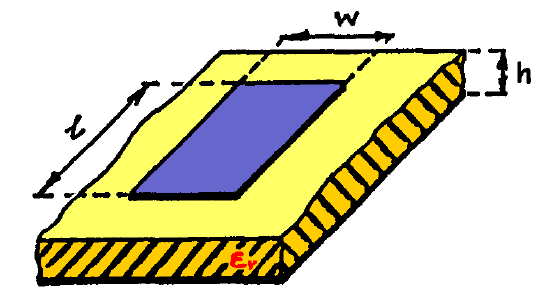
\includegraphics[scale=0.435]{Obrazky/MVT/planarny_rezonator.png}}
		\caption{Obdĺžnikový deskový rezonátor}
	\end{figure}


	
	
	\section{Dielektrický rezonátor} \label{rez:dielec_rezon}
	\begin{itemize}[label=--]
		%\vspace*{-3mm}
		\item mikrovlnný rezonančný prvok tvorený materiálom s nízkymi stratami (keramické dielektrikum napr.)
		%\vspace*{-3mm}
		\item vysoká relatívna permitivita $\epsilon_r$ $\rightarrow$ pole je tak uchované vo vnútri objektu, malé rozptylové pole na hranách
		%\vspace*{-3mm}
		\item tvary: válec/kváder
		%\vspace*{-3mm}
		\item vysoký činiteľ jakosti Q (straty dané iba stratami v dielektriku)
	\end{itemize}
	
	\subsubsection{Výhody dielektrických rezonátorov}
	%\vspace*{-2mm}
	\begin{itemize}[label=$\oplus$]
		\item Malé rozmery (10$\times$ $\approx$ 20$\times$ menší než dutinové rezonátory - $c/\sqrt{\epsilon_r}$ - môžu byť menšie)
		%\vspace*{-3.5mm}
		\item Vysoký činiteľ jakosti (nenastávajú straty vo vodivých stenách, vyžarovanie veľmi malé)
		%\vspace*{-3.5mm}
		\item Vysoká teplotná stabilita - dôvod: keramické materiály pre rezonátory
	\end{itemize}
	
	\begin{figure}[H]
		\makebox[\textwidth]{%
			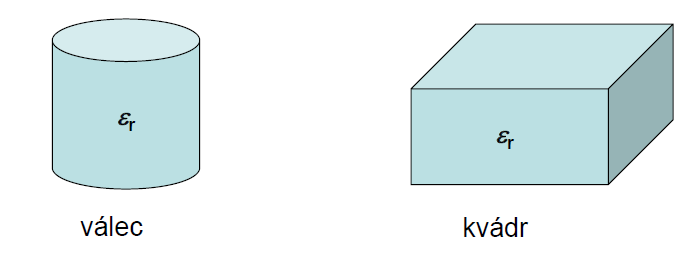
\includegraphics[scale=0.435]{Obrazky/MVT/dielektricke_rezonatory.png}}
		\caption{Dielektrické rezonátory}
	\end{figure}
	
	
	
	
	\section{Budenie vlnovodu a dutinových rezonátorov} \label{budenie:vlnovod:dutin}
	\subsubsection{Budenie prúdovou sondou}
	\begin{itemize}[label=--]
		%\vspace*{-3mm}
		\item realizuje sa krátkym úsekom vodiča (napr. stredným vodičom koaxiálneho vedenia) dĺžky~$h\ll~\lambda$ zasunutím do budeného vlnovodu či dutinového rezonátora. 
		%\vspace*{-4mm}
		\item pre optimálne budenie určitého vidu elmag. poľom musí platiť:
		\begin{itemize}[label=$\rightarrow$]
			%\vspace*{-3mm}
			\item \textbf{Orientácia sondy} -- sonda zasunutá rovnobežne so siločiarami el. poľa budené vidu
			%\vspace*{-6.5mm}
			\item \textbf{Umiestnenie sondy} -- sonda zasunutá v mieste maximálnej intenzity el. poľa budeného vidu
			%\vspace*{-1.5mm}
			\item \textbf{Kmitočet zdroja} -- frekvencia budiaceho signálu vyššia než medzný kmitočet
			%\vspace*{-1.5mm}
			\item Veľkosť budenia čiastočne ovplyvnené zmenou hĺbky zasunutia sondy
		\end{itemize}
		%\vspace*{-5.5mm}
		\item na princípu budenia prúdovou sondou je konštruovaná väčšina prechodov koax. -- vlnovod
		%\vspace*{-8mm}
		\item \textbf{budenie dominantného vidu} TE$_{10}$ obdĺžnikového vlnovodu, ktorý je na jednom konci skratovaný, budiací kmitočet by mal ležať v pásme jednovidovosti daného vlnovodu
		\end{itemize}
	
	\subsubsection{Budenie magnetickou slučkou}
	\begin{itemize}[label=--]
		%\vspace*{-3mm}
		\item prúdová sonda je vytvarovaná do malej ,,takmer uzavretej'' slučke
		%\vspace*{-4mm}
		\item pre optimálne budenie určitého vidu vo vlnovode či v dutinovom rezonátore musí byť:
		\begin{itemize}[label=$\rightarrow$]
			%\vspace*{-3mm}
			\item \textbf{Orientácia slučky} -- plocha slučky kolmá k mag. siločiarám vidu
			%\vspace*{-2mm}
			\item \textbf{Umiestnenie slučky} -- stred slučky v mieste max. intenzity mag. poľa
			%\vspace*{-2mm}
			\item \textbf{Kmitočet zdroja} -- opäť frekvencia budiaceho signálu vyššia než medzný kmitočet
			%\vspace*{-7mm}
			\item Veľkosť budenia je možné reagovať od nuly až do maximálnej hodnoty natáčaním plochy slučky o uhol \qty{90}{\degree}
		\end{itemize}
		%\vspace*{-5mm}
		\item na princípe budenia magnetickou slučkou sú konštruované prechody koax. -- pravoúhlý vlnovod (axiálne prechody)
	\end{itemize}
	
	\subsubsection{Budenie väzobným otvorom (šterbinou)}
	\begin{itemize}[label=--]
		%\vspace*{-3mm}
		\item v kovovej stene vlnovodu/dutinového rezonátoru je vyrezaný malý väzobný otvor
		%\vspace*{-3mm}
	    \item vo väzobnom otvore sa z vonku vytvorí budiace elektrické pole (vonkajším vedením, vonkajším vlnovodom alebo ožiarením elektromag. vlnou), ktorým je budený požadovaný vid v budenom vlnovode/rezonátore 
		%\vspace*{-3mm}
		\item pre optimálne budenie musí platiť:
		\begin{itemize}[label=$\rightarrow$]
			%\vspace*{-3mm}
			\item \textbf{Orientácia el. poľa} -- budiace el. pole vo šterbine kolmé na smer magnetických siločiar budeného vidu
			%\vspace*{-2mm}
			\item \textbf{Umiestnenie šterbiny} -- stred šterbiny v mieste max. magnetického poľa budeného vidu
			%\vspace*{-2mm}
			\item \textbf{Kmitočet zdroja} -- frekvencia budiacého signálu vyššia než medzný kmitočet
			%\vspace*{-1.25mm}
			\item Veľkosť budenia je možné regulovať od nuly až do maximálnej hodnoty natáčaním plochy slučky o uhol \qty{90}{\degree} 
		\end{itemize}
		%\vspace*{-4.5mm}
		\item na princípe budenia magnetickou slučkou sú konštruované prechody koax. -- pravoúhlý vlnovod (axiálne prechody)
	\end{itemize}
	
	\begin{figure}[H]			
		\centering
		\begin{subfigure}[t]{0.48\textwidth}
			\centering
			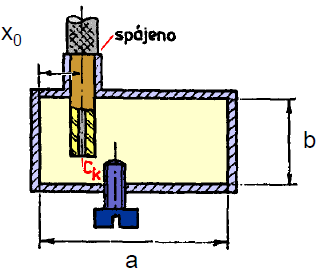
\includegraphics[scale=0.3]{Obrazky/MVT/budenie_prud_sonda.png}
			\caption{prechod koax. -- vlnovod}
		\end{subfigure}
		\hspace{-20mm}
		\begin{subfigure}[t]{0.48\textwidth}
			\centering
			\captionsetup{justification=centering}
			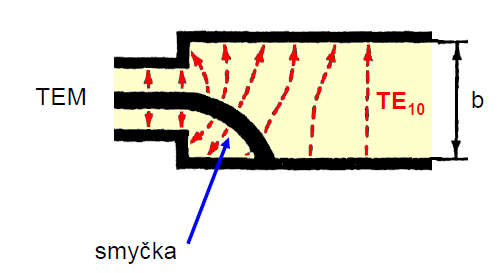
\includegraphics[scale=0.3]{Obrazky/MVT/budenie_mag_slucka.png}
			\caption{prechod koax. -- pravoúhlý vlnovod}
		\end{subfigure}
		\caption{Prechody budenia}
		\label{fig:prechody}
	\end{figure}
	
	%\vspace*{-10mm}
%	\section{\normalsize \begin{itemize}\item[3.] \hyperref[delice]{Výkonové děliče}, \hyperref[odbnocnice]{směrové vazební členy} a jejich \hyperref[odbnocnice_param]{základní technické parametry}.\end{itemize}} \label{delice}
	\section{3. Okruh}
	%\vspace*{-0mm}
	\begin{itemize}[label=--]
		%\vspace*{-2mm}
		\item výkonové deliče a smerové odbočnice sú pasívne mikrovlnné komponenty pre delenie nebo zlučovanie signálov
	\end{itemize}	
	%\vspace*{-5mm}
	\begin{figure}[H]
		\makebox[\textwidth]{%
			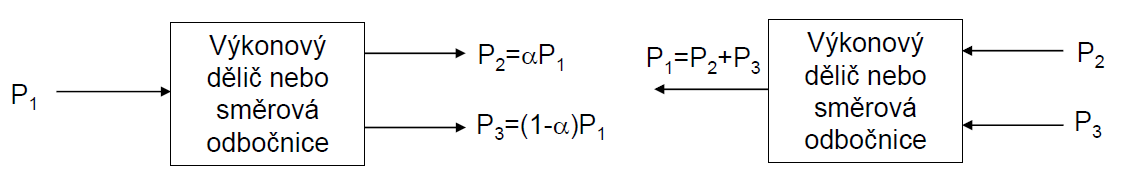
\includegraphics[scale=0.3]{Obrazky/MVT/vykonovy_delic_smer_odbocnica.png}}
		\caption{Výkonové deliče a smerové odbočnice}
	\end{figure}
	%\vspace*{-8mm}
	
	\subsubsection{Výkonový delič typ T}
	\begin{itemize}[label=--]
		%\vspace*{-2mm}
		\item je jednoduchý trojbran, ktorý môže byť použitý k rozdeleniu alebo zlúčeniu signálu
		%\vspace*{-3.5mm}
		\item môže byť vytvorený na základe akéhokoľvek vedenia 
		%\vspace*{-3.5mm}
		\item reciproký trojbran nemôže byť zároveň bezstrstovy a ideálne prispôsobený na všetkých svojich bránach
	\end{itemize}
		
	\begin{figure}[H]
		\captionsetup{justification=centering}
		\makebox[\textwidth]{%
			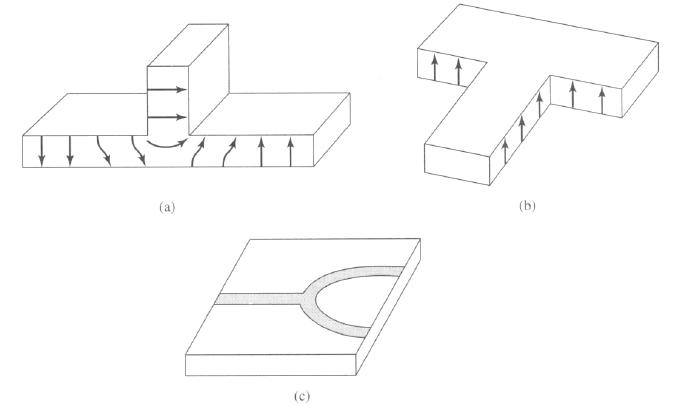
\includegraphics[scale=0.4]{Obrazky/MVT/t_junctions.png}}
		\caption{a.) T-spojenie vlnovodu v E-rovine, b.) T-spojenie vlnovodu v H rovine, c.)~T-spojenie mikropáskových vedení}
	\end{figure}		
		
		
	\subsubsection{Wilkinsonov delič výkonu}
	\begin{itemize}[label=--]
		%\vspace*{-2mm}
		\item rozdeľuje výkon rovnakým dielom z jedného vstupného vedenia s char. impedanciou $Z_0$ na $n$ výstupných vedení o rovnakej charakteristickej impedancii
		%\vspace*{-3.5mm}
		\item výstupný signál má rovnakú fázu
		%\vspace*{-3.5mm}
		\item výstupné brány sú medzi sebou izolované
		%\vspace*{-3.5mm}
		\item \textbf{princíp izolácie:}
		\begin{itemize}[label=$\rightarrow$]
			%\vspace*{-3mm}
			\item signál z jednej brány do druhej sa šíri dvoma cestami
			%\vspace*{-2mm}
			\item jedna cesta je cez odpor, ktorý funguje ako izolátor brán (ak by došlo k odrazu signálu späť do deliča, rezistor pohltí tento signál)
			%\vspace*{-2mm}
			\item druhá cesta je cez 2 štvrťvlnné úseky vedení (zmena fázy o \qty{180}{\degree}) $\rightarrow$ oba signály sa pred vstupom do portu vynulujú)
		\end{itemize}
		%\vspace*{-5mm}
		\item môže byť použitý (po modifikácií) aj pre nerovnomerne delenie výkonu (s iným pomerom)
		%\vspace*{-8.5mm}
		\item pri n-bránach deliča sa používa pre vedenia $\lambda/4$ impedancia $\sqrt{N}Z_0$, kde N je počet $\lambda/4$ vedení
	\end{itemize}

	\begin{figure}[H]
		\captionsetup{justification=centering}
		\makebox[\textwidth]{%
			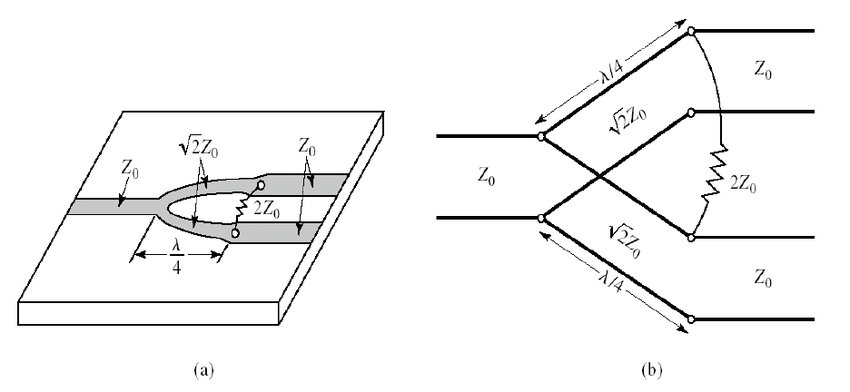
\includegraphics[scale=0.375]{Obrazky/MVT/willkinson_delic.png}}
		\caption{a.) Wilkinsonov delič na doske, b.) ekvivalentné zapojenie Wilkinsonovho deliča}
	\end{figure}	

	\subsubsection{Smerové väzobné členy (smerové odbočnice)} \label{odbnocnice}
		\begin{itemize}[label=--]
		%\vspace*{-2mm}
		\item pasívna mikrovlnná súčiastka (podskupina deličov)
		%\vspace*{-3mm}
		\item ich úlohou je odbočiť malú časť signálu z hlavnej trasy (z portu 1 do portu 2) do vedľajšej vetvy (port 3)
		%\vspace*{-3mm}
		\item dokáže rozlíšiť smer šírenia vlny:
		\begin{itemize}[label=$\rightarrow$]
			%\vspace*{-3mm}
			\item dopredná vlna (priama)
			%\vspace*{-2mm}
			\item odrazená vlna
		\end{itemize}
		%\vspace*{-4mm}
		\item požaduje sa, aby týmto odbočením sa do hlavného vlnovodu nevniesli \textbf{prídavné odrazy} a aby, zmeny pracovných pomerom vo vedľajšej vetvy \textbf{neovplyvňovali hlavnú vetvu}
		%\vspace*{-3mm}
		\item \textbf{ideálna smerová odbočnica}: každý bezstratový, recipročný a totálne prispôsobený štvorbrán
	\end{itemize}
	
	\begin{figure}[H]
		\captionsetup{justification=centering}
		\makebox[\textwidth]{%
			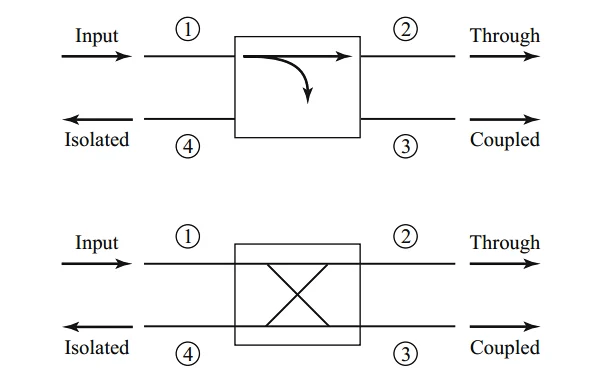
\includegraphics[scale=0.35]{Obrazky/MVT/directional_coupler.png}}
		\caption{Smerová odbočnica}
	\end{figure}
	
	\subsubsection{Základné param. smerových odbočníc} \label{odbnocnice_param}
	{\raggedright
	\textbf{Väzobný útlm -- coupling C} - (jak veľká časť signálu odbočí zo vstupu do odbočky)}
	\begin{equation}
		C = 10 \log \frac{P_1}{P_{13}} \text{    [dB]}
	\end{equation}
	
	{\raggedright
	\textbf{Priechodzí (vložený) útlm -- insertion loss - IL} - (strata výkonu medzi vstupom (port 1) a výstupom (port 2))}
	\begin{equation}
		IL = 10 \log \frac{P_1}{P_{12}} \text{    [dB]}
	\end{equation}
	
	{\raggedright
	\textbf{Izolácia -- isolation - I} - (oddelenenie záťaže (port 1) a odbočky (port 3))}
	\begin{equation}
		I = 10 \log \frac{P_1}{P_{14}} = 10 \log \frac{P_2}{P_{23}} \text{    [dB]}
	\end{equation}
	
	{\raggedright
	\textbf{Smerovosť -- directivity - D} - (vyjadruje dokonalosť oddelenia priamej a odrazenej vlny, pri ideálnej odbočnici \textbf{D} = $\infty$)}
	\begin{equation}
		D = 10 \log \frac{P_{13}}{P_{14}} = 10 \log \frac{P_{13}}{P_{23}} \text{    [dB]}
	\end{equation}
	
	{\raggedright
	\textbf{Zpätný útlm -- return loss - RL} - (určuje aká časť výkonu sa odrazí od vstupu späť}
	\begin{equation}
	RL = 10 \log \frac{P_1}{P_{1odraz}} = 10\log{\frac{1}{\abs{\rho}^2}} = 20 \log {\frac{1}{\abs{\rho}}} \text{    [dB]}
	\end{equation}
	
	\section{Typy vlnovodových odbočníc:}
	\subsubsection{Betheova smerová odbočnica}
	\begin{itemize}[label=--]
		%\vspace*{-2mm}
		\item elektrická väzba medzi vlnovody nezávisí na úhle $\psi$, magnet. väzba je úmerná hodnote~$\cos\psi$
		%\vspace*{-3.5mm}
		\item pre (\ref{eq:dokonale_izol}) je brána 4 dokonale izolovaná
		%\vspace*{-3.5mm}
		\item pre $\psi = 90^\circ$ stráca odbočnica svoje smerové vlastnosti a brány 3 a 4 sú rovnako budené
		%\vspace*{-3.5mm}
		\item pre $\psi = 0^\circ$ má odbočnica smerové vlastnosti len pri $\lambda_0 = 1,41a$
		%\vspace*{-3.5mm}
		\item \textbf{nevýhoda}: nie je možné vytvoriť jedným väzobným otvorom silnou väzbou 
	\end{itemize}
	
	\begin{equation}
		1 - \left( \frac{\lambda}{2a} \right)^2 = \frac{1}{2 \cos \psi}
		\label{eq:dokonale_izol}
	\end{equation}
	
	\begin{figure}[H]
		\captionsetup{justification=centering}
		\makebox[\textwidth]{%
			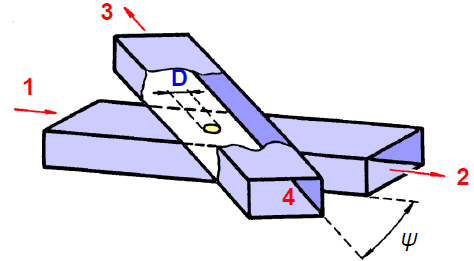
\includegraphics[scale=0.4]{Obrazky/MVT/betheova_smerova_odbocnica.png}}
		\caption{Betheova smerová odbočnica}
	\end{figure}
	\newpage
	
	\subsubsection{Odbočnica s niekoľko väzobnými otvormi}
	
	\begin{itemize}[label=--]
		%\vspace*{-2mm}
		\item princíp vychádza zo skladania vzájomne fázovo posunutých vĺn pri šírení medzi väzobnými otvormi
		%\vspace*{-3.5mm}
		\item sčítania vĺn s rovnakou fázou (ich aplitúda sa sčíta) a sčítanie vĺn vzájomne fázovo posunutých (vyruší sa) 
	\end{itemize}
	
	\subsubsection{Odbočnica s dvoma otvormi vzdialenými o $\mathbf{\lambda_g/4}$:}
	\begin{itemize}[label=--]
	\item 2 vlnovody (hlavný a odbočný) sú spojené spoločnou stenou s malými otvormi vzdialenými o $\lambda_g/4$
	%\vspace*{-3.5mm}
	\item časť presiaknutých vĺn v oboch otvoroch sa navzájom sčíta a na porte 3 nameriame ich výkon
	%\vspace*{-3.5mm}
	\item časť presiaknutých vĺn putuje aj smerom k portu 4 $\rightarrow$ tieto vlny sú voči sebe posunuté o $2 \times \lambda_g/4 = 180\degree$ a navzájom sa vyrušia
	%\vspace*{-3.5mm}
	\item \textbf{nevýhoda}: značná kmitočtová závislosť smerovej odbočnice
	\end{itemize}

	\begin{figure}[H]
		\captionsetup{justification=centering}
		\makebox[\textwidth]{%
			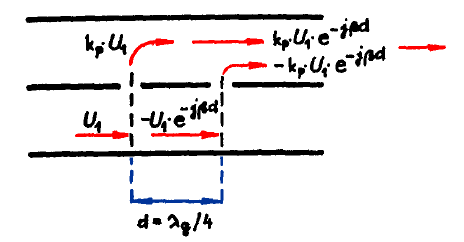
\includegraphics[scale=0.4]{Obrazky/MVT/odbocnice_lambda_g_4.png}}
		\caption{Odbočnica s dvoma otvormi vzdialenými o $\lambda_g/4$ (vlna smeruje do portu 3)}
	\end{figure}
	
	\subsubsection{Odbočnica se dvoma otvory vzdialenými o $\mathbf{\lambda_g/4}$ s opačnou fázou:}
	\begin{itemize}[label=--]
		\item  tvarovaním druhého otvoru docielime, že vlna prechádzajúca týmto otvorom spraví fázový posun 180 \degree\ a vyruší vlnu smerujúcu do portu 3 $\rightarrow$ dopredné vlny sa vyrušia, vlny smerujúce späť (do portu 4) sa navzájom sčítajú
		%\vspace*{-3.5mm}
		\item napr. Schwingerova odbočnica, Ribletova odbočnica
	\end{itemize}
	
	\begin{figure}[H]
		\captionsetup{justification=centering}
		\makebox[\textwidth]{%
			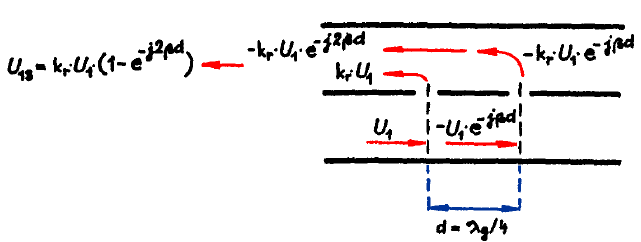
\includegraphics[scale=0.4]{Obrazky/MVT/odbocnice_lambda_g_4_opacna.png}}
		\caption{Odbočnica s dvoma otvormi vzdialenými o $\lambda_g/4$: s opačnou fázou\\(vlna smeruje do portu 4)}
	\end{figure}
	
	\subsubsection{Odbočnica s jedným veľkým väzobným otvorom (príp. s veľa väzobnými otvormi)}
	\begin{itemize}[label=--]
		\item je možné realizovať aj slabú aj silnú väzbu, má vysokú smerovosť a veľkú šírku pásma
		%\vspace*{-3.5mm}
		\item mnohošterbinové vlnovodové odbočnice $\rightarrow$ najdokonalejšie a najvyužívanejšie typy
	\end{itemize}
	
	\begin{figure}[H]
		\captionsetup{justification=centering}
		\makebox[\textwidth]{%
			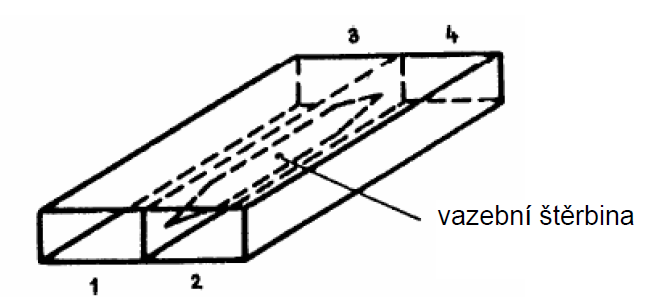
\includegraphics[scale=0.4]{Obrazky/MVT/mnohosterbinove_odbocnice.png}}
		\caption{Mnohošterbinová odbočnica}
	\end{figure}
	
\subsubsection{Odbočnica z viazaných vedení}
\begin{itemize}[label=--]
	%\vspace*{-2mm}
	\item pri umiestnení dvoch netienených prenosových vedení blízko seba vzniká elektromagnetická väzba medzi vedeniami
	%\vspace*{-3mm}
	\item väzba vzniká v dôsledku interakcie elektromagnetických polí jednotlivých vedení
	%\vspace*{-3mm}
	\item smerové vlastnosti smerovej odbočnice vznikajú superpozíciou vybudených vidov elektromagnetického poľa
	%\vspace*{-3mm}
	\item fázové pomery sú navrhnuté tak, aby sa v jednom výstupnom ramene vlny sčítali
	%\vspace*{-3mm}
	\item v izolovanom ramene sa vlny navzájom vyrušia
\end{itemize}
	
	\begin{figure}[H]
		\captionsetup{justification=centering}
		\makebox[\textwidth]{%
			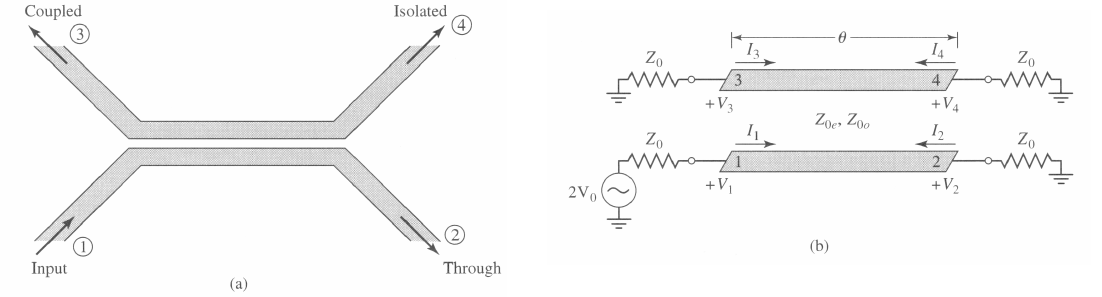
\includegraphics[scale=0.4]{Obrazky/MVT/odbocnice_viazane_vedenia.png}}
		\caption{Odbočnice z viazaných vedení}
	\end{figure}
	
%\end{document}



 